\section{Introduzione}


% METODI DI MISURA DIRETTA
\begin{frame}{Neve come risorsa idrica}
  
  \centering
  \vspace{5pt}
  {\large\bfseries\boldmath Manto nevoso $\Rightarrow$ risorsa idrica\par}
  \begin{columns}[T, onlytextwidth]

    \begin{column}{0.48\textwidth}
      \begin{block}{Misure in-situ}
        \footnotesize
        \begin{itemize}[label=$\blacktriangleright$]
          \item Network poco denso
          \item focus su spessore nevoso
        \end{itemize}

        \parbox[c][0.5\textheight][c]{\linewidth}{\centering
          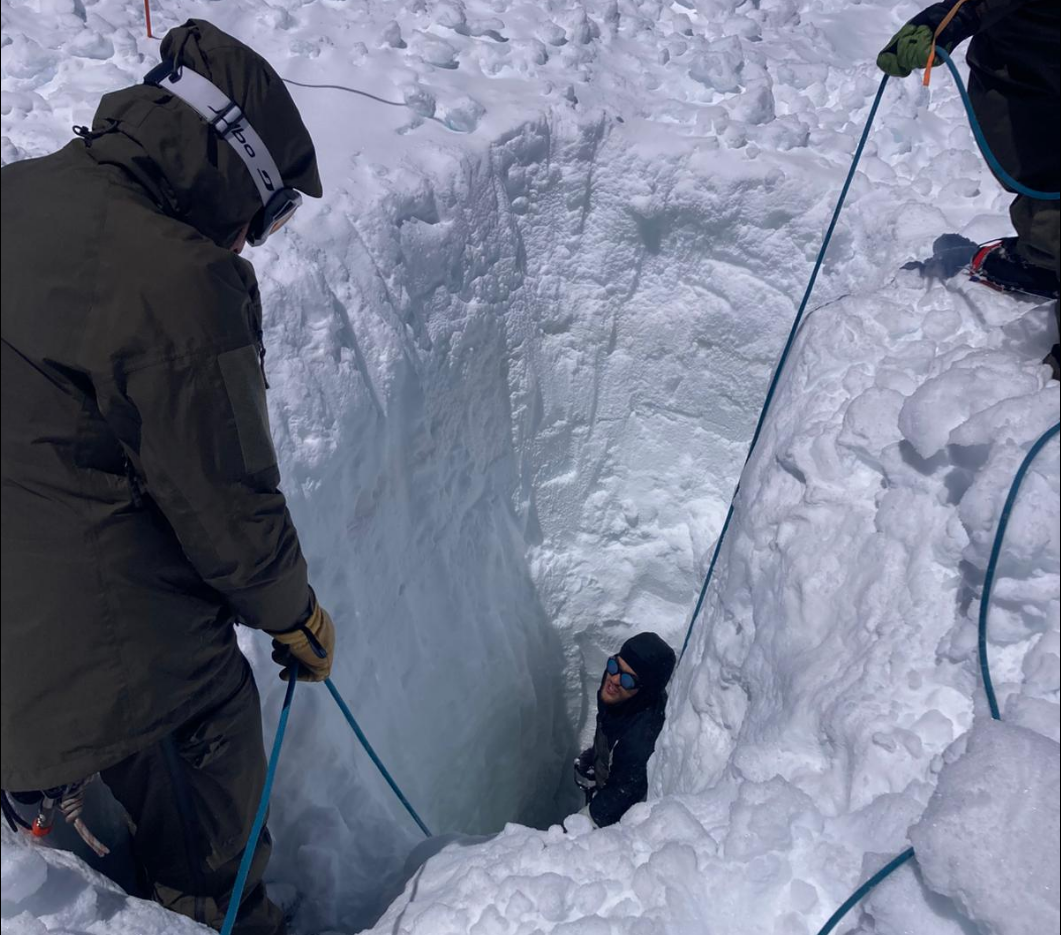
\includegraphics[width=\linewidth, height=0.5\textheight, keepaspectratio]{images/introduzione/snow_pit.png}}
      \end{block}
    \end{column}

    \begin{column}{0.48\textwidth}
      \begin{block}{Misure satellitari}
        \footnotesize
        \begin{itemize}[label=$\blacktriangleright$]
          \item Misure spazializzate
          \item risoluzione $\leftrightarrow$ copertura temporale
        \end{itemize}

        \parbox[c][0.5\textheight][c]{\linewidth}{\centering
          \includegraphics[width=\linewidth, height=0.5\textheight, keepaspectratio]{example-image-b}}
      \end{block}
    \end{column}

  \end{columns}

\end{frame}


% MODELLI NUMERICI
\begin{frame}{Metodi di stima}

  \begin{columns}[T, onlytextwidth]

    \begin{column}{0.48\textwidth}
      \centering
      {\usebeamercolor[fg]{structure}\bfseries IT-SNOW\par}
      \medskip
      \begin{minipage}[t][0.25\textheight][t]{\linewidth}
        \raggedright\small
        \begin{itemize}[label=$\blacktriangleright$]
          \item Network poco denso
          \item SWE raramente misurato (focus su spessore nevoso)
        \end{itemize}
      \end{minipage}

      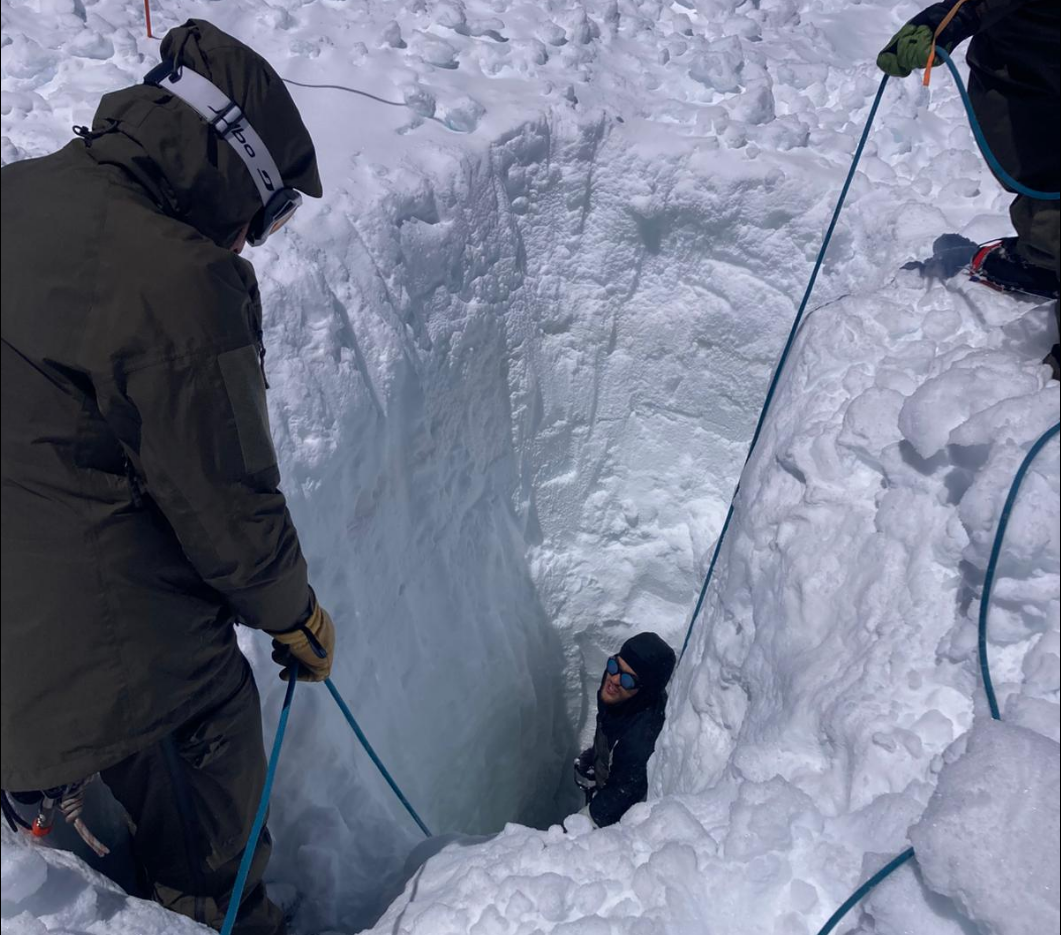
\includegraphics[width=\linewidth, height=0.5\textheight, keepaspectratio]{images/introduzione/snow_pit.png}
    \end{column}

    \begin{column}{0.48\textwidth}
      \centering
      {\usebeamercolor[fg]{structure}\bfseries Po River District\par}
      \medskip
      \begin{minipage}[t][0.25\textheight][t]{\linewidth}
        \raggedright\small
        \begin{itemize}[label=$\blacktriangleright$]
          \item Misure spazializzate
          \item Trade-off risoluzione-copertura temporale
        \end{itemize}
      \end{minipage}

      \includegraphics[width=\linewidth, height=0.42\textheight, keepaspectratio]{example-image-b}
    \end{column}

  \end{columns}

\end{frame}